%%%%%%%%%%%%%%%%%%%%%%%%%%%%%%%%%%%%%%%%%%%%%%%%%%%%%%%%%%%%%%%%%%%%%%%%%%%%%%%
% bc.tex - Bachelor thesis                                                    %
% Subject: bc_emu - portable video game emulator                              %
% Chapter: Specifikace                                                        %
% Author: Ondrej Balaz <ondra@blami.net>                                      %
%%%%%%%%%%%%%%%%%%%%%%%%%%%%%%%%%%%%%%%%%%%%%%%%%%%%%%%%%%%%%%%%%%%%%%%%%%%%%%%

\chapter{NEC PCEngine}\label{chap:spec}

Znalost principů fungování emulovaného systému a systému samotného je jedním z
klíčových předpokladů pro úspěšnou implementaci emulátoru. U videoherních
systémů je získání technické specifikace většinou obtížné, protože se jedná o
uzavřené produkty a jejich výrobci mají komerční a jiné důvody, proč oficiální
dokumentaci nezveřejňovat a to dokonce i v době, kdy pro ně konkrétní systém už
nemá žádný komerční význam.

Autoři emulátorů jsou tak odkázání na metody reverzního
inženýrství\footnote{Snaha o odkrytí principu na kterém funguje zařízení, např.
za účelem jeho chování napodobit.}, přičemž vzniká často používaná neoficiální
dokumentace, která, i přes svůj přínos, může být neúplná nebo nepřesná. V
případě systému NEC PCEngine tento proces navíc komplikuje malá popularita a
tedy i malý počet zainteresovaných vývojářů a fakt, že jeho výrobce šel cestou
použití zcela specifického hardware (ostatní systémy téže generace byly téměř
bez výhrady postaveny na dobře zdokumentovaných procesorech MOS 6502 či Zilog
Z80).

Sekce~\ref{chap:spec_history}, která otevírá tuto kapitolu, stručně představuje
videoherní systém NEC PCEngine a stručně pojednává o jeho historii.

Protože pravděpodobně neexistuje žádný dokument, který by shrnoval dostupné
technické specifikace základní verze systému NEC PCEngine na jednom místě, ale
jen dílčí dokumenty specializující se na technickou specifikaci určité částí
systému NEC PCEngine, je v sekci~\ref{chap:spec_hw} předložena co možná
nejkompletnější\footnote{Z hlediska specifik systému NEC PCEngine, pro
přehlednost není uvedena např. kompletní specifikace procesoru WDC 65c02 z nějž
vychází procesor HuC6280 použitý v systému NEC PCEngine, ale jen odlišnosti
použitého procesoru HuC6280.} specifikace tohoto systému, která je založena
nejen na zmiňovaných dokumentech~\cite{Ormston06, MacDonald02, Schleussinger98,
Clifford, Woodford94, LaMothe05, www65c02}, ale také na studiu zdrojových kódů
existujících emulátorů \cite{wwwMednafen, wwwOotake} a konečně i vlastních
zkušenostech nabytých při implementaci emulátoru.

Poslední sekce~\ref{chap:spec_sw} této kapitoly pak stručně pojednává o
software dostupném pro systém NEC PCEngine.

% -----------------------------------------------------------------------------
% Historie
% -----------------------------------------------------------------------------

\section{Historie}\label{chap:spec_history}

NEC PCEngine je hybridní videoherní konzole vyvinutá japonskými společnostmi
HudsonSoft a NEC v roce 1987. Hybridní je nazývána proto, že ačkoliv hlavní
procesor je 8-mi~bitový, jako u většiny herních konzolí 3. generace
(Nintendo Famicom, Sega Master System, Atari 7800), grafický systém je plně
16-ti bitový. Vzhledem k tomu, že NEC PCEngine bylo uvedeno do prodeje v roce
1987, NEC předběhl své hlavní rivaly v použití 16-ti bitové technologie a z ní
vyplývajících výhod o celou jednu generaci herních konzolí. Pokročilý 6-ti
kanálový zvukový subsystém dovoloval kromě přehrávání samplů i jednoduchou
zvukovou syntézu a modulaci zvuku. Je jen s podivem, že tak pokročilý systém,
jakým bezesporu ve své době NEC PCEngine byl, zdaleka nedosáhl světové obliby
na alespoň stejné úrovni jako ostatní videoherní konzole téže
generace.~\cite{wwwClassicGaming, wwwWikiTurboGrafx}

\begin{figure}[ht]
\begin{center}
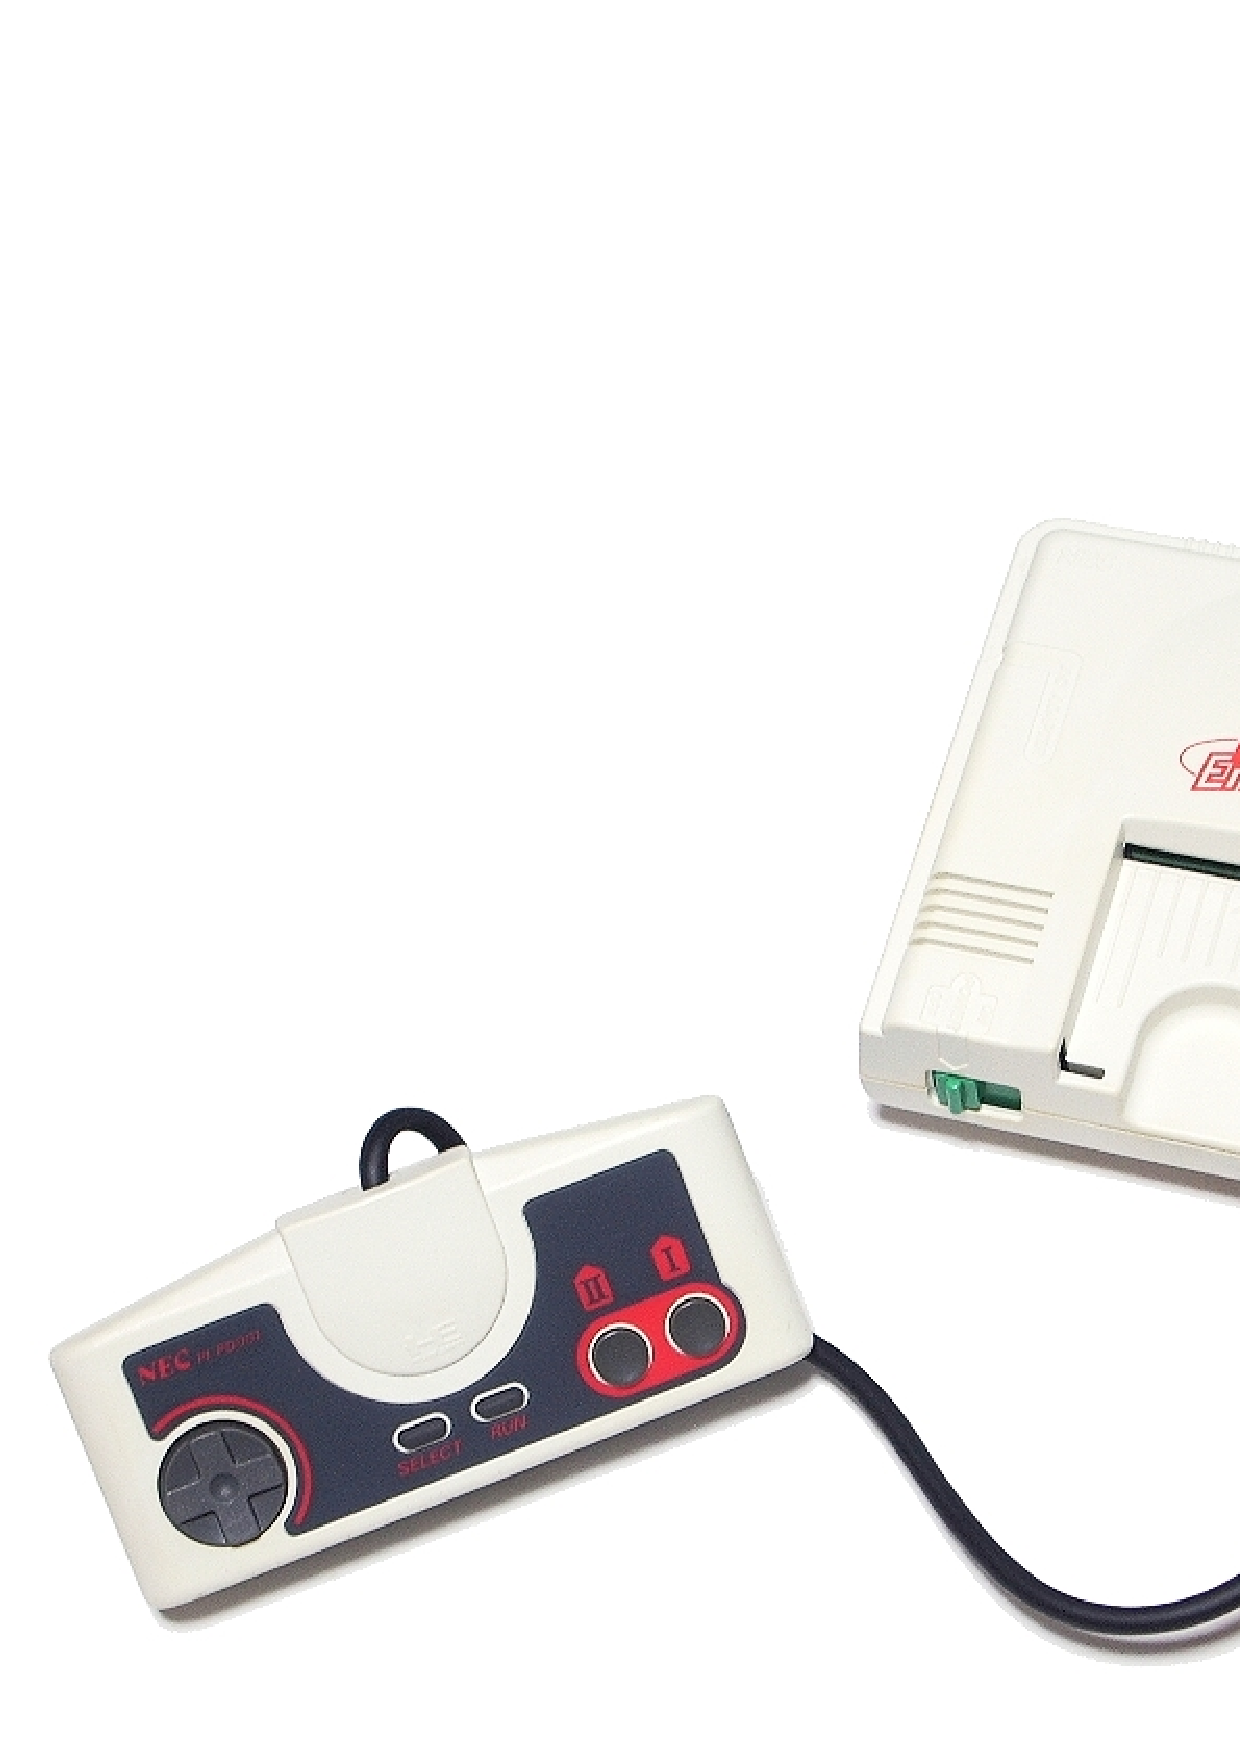
\includegraphics[width=6cm]{fig/pce_photo}
\caption{Systém NEC PCEngine, základní varianta\label{fig:pce_photo}}
\end{center}
\end{figure}

Systém NEC PCEngine byl firmou NEC postupně inovován. Kromě rozšíření paměti a
přidání vstupního portu pro další herní ovladač(e) se v následujících verzích
dočkala i rozšíření (jako první videoherní konzole na světě) o CD-ROM jednotku
a další grafický koprocesor. Mírně modifikovaný systém byl od roku 1989 v malém
nákladu exportován z Japonska do Severní Ameriky a Evropy pod názvem NEC
TurboGrafx 16, kde se ale vůbec neprosadil vlivem špatného marketingu a
nedostatku vývojářů her. {\em Pozn.: popsaná rozšíření ani modifikace nejsou v
práci uvažovány.}~\cite{wwwClassicGaming, BartonLoguidice09}

S příchodem plně 16-ti bitových herních konzolí 4. generace (Sega Genesis,
Super Nintendo Entertainment System) v roce 1991 přišel systém NEC PCEngine o
své místo na trhu a po neúspěších s dalším systémem (PC FX32) opouští NEC
videoherní průmysl.~\cite{wwwWikiTurboGrafx}

Zajímavostí pro doplnění je, že svými fyzickými rozměry 14cm x 14cm x 3.8cm se
NEC PCEngine zapsalo do Guinnessovy knihy rekordů jako nejmenší nepřenosná
videoherní konzole.~\cite{Guinness08}

% -----------------------------------------------------------------------------
% Hardware NEC PCEngine
% -----------------------------------------------------------------------------

\section{Hardware}\label{chap:spec_hw}

Základní verze NEC PCEngine je vybavena 8~KB operační paměti (RAM) a 64~KB
videopaměti (VRAM). Hlavní procesor HuC6280 řídí zpracování programu uloženého
v paměti určené pouze pro čtení (ROM) na výměnné čipové kartě
HuCard\footnote{Čipové karty HuCard měly formát kreditní karty, čímž se zásadně
lišily od podstatně větších zásuvných modulů rivalských systémů od společností
Nintendo a Sega.}. Dále zajišťuje ozvučení programu pomocí programovatelného
generátoru zvuků (Programmable Sound Generator, PSG) o 6ti kanálech a
zpracování vstupu z portu herního ovladače.

O obrazový výstup se stará dvojice 16-ti bitových grafických pomocných
procesorů, konkrétně kontrolér pro zobrazování (Video Display Controller, VDC)
HuC6270 a enkodér barev (Video Color Encoder, VCE) HuC6260. Ty společně
zajišťují zobrazení v rozlišeních až 512x240 pixelů v 9-ti bitové barevné
hloubce (512 barev celkem, na obrazovce zobrazitelných maximálně 482 barev)
pomocí RF (anténního) výstupu na televizní set ve standardu NTSC.~\cite{wwwWikiTurboGrafx}

%
% CPU
%

\subsection{CPU}\label{chap:spec_hw_cpu}

Hlavní procesor celého systému (Central Processing Unit, CPU) nese označení
HuC6280 a vychází z mikroprocesoru WDC 65c02 společnosti Western Digital, jehož
specifikaci~\cite{www65c02} rozšiřuje o řadu instrukcí a adresních módů a
přidává některá, pro účely videoherního systému, specifická periferní zařízení.
Jedná se o 8-mi bitový procesor schopný operovat na frekvencích 3.58~MHz a
7.16~MHz (lze libovolně měnit za běhu programu vykonáním dvou speciálních
instrukcí {\sc csl} a {\sc csh}). Architektura systému je znázorněna na
obr.~\ref{fig:pce_arch}.

\begin{figure}[ht]
\begin{center}
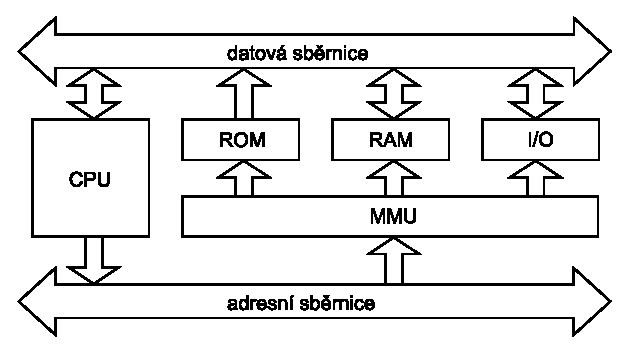
\includegraphics[width=10cm,height=5.3cm]{fig/pce_arch}
\caption{Architektura systému NEC PCEngine\label{fig:pce_arch}}
\end{center}
\end{figure}

Z hlediska endianity je CPU HuC6280 \uv{little-endian}\footnote{Při práci s
vícebajtovými položkami je nejméně významný bajt je v paměti uložen na nejnižší
adrese.}. Tento fakt se pochopitelně týká i obou grafických pomocných procesorů
VDC HuC6270 a VCE HuC6260. V následujícím textu se s touto skutečností mlčky
počítá.

Jak již bylo zmíněno, oproti WDC 65c02 disponuje CPU HuC6280 řadou periferních
zařízení: jednotkou obsluhy přerušení, 8-mi bitovým paralelním I/O portem (pro
herní ovladač), jednotkou správy paměti (mapovačem), časovačem a
programovatelným generátorem zvuku (PSG).

% Registry

\subsubsection{Registry}\label{chap:spec_hw_cpu_reg}

\begin{description}
\item[{\sf A}] Střadač (Accumulator) \\
	Bezpochyby nejdůležitější registr CPU HuC6280. Slouží jako zdrojový, cílový
	nebo oba operandy pro většinu instrukcí. Je to jedinný registr, který lze
	použít s řadou insturkcí pro provádění matematických výpočtů. Délka
	registru {\sf A} je 8 bitů.

\item[{\sf X}] Indexový registr X (Index X) \\
	Jedná se o registr obecného použití často využívaný při některých adresních
	módech s nepřímou adresou. Je též používán jako vnitřní čítač pro cykly.
	Délka registru {\sf X} je 8 bitů.

\item[{\sf Y}] Indexový registr Y (Index Y) \\
	Jedná se opět o registr obecného použítí s podobným využitím a vlastnostmi
	jako má registr {\sf X}. Délka registru {\sf Y} je 8 bitů.

\item[{\sf PC}] Čítač programu (Program counter) \\
	Obsahuje adresu instrukce, která se má vykonat. Ve chvíli kdy dojde k
	vykonání instrukce je hodnota čítače automaticky
	zvýšena/změněna\footnote{Ke změnám, které nemusí být inkrementací dochází
	např. při použití instrukcí skoku nebo volání podprogramu.}. Délka registru
	{\sf PC} je 16 bitů.

\item[{\sf S}] Ukazatel na zásobník (Stack pointer) \\
	Obsahuje adresu prvního volného místa v zásobníku\footnote{Místo v paměti
	určené k dočasným odložení hodnot programem.}. Délka registru {\sf S} je 8
	bitů.

\item[{\sf P}] Příznakový registr (Program flags) \\
	Tento velice významný registr obsahuje bitové pole s příznaky indikujícími
	aktuální stav procesoru po poslední provedené operaci. Některé z těchto
	příznaků mohou být i nastaveny z programu. Jednotlivé příznaky jsou uvedeny
	v tabulce~\ref{tab:cpu_flags}. Význam jednotlivých příznaků následuje.

	\begin{table}[ht]
	\begin{center}
	\begin{tabular}{|c|c|c|c|c|c|c|c|c|}
	\hline
	\textbf{Bit} & 7 & 6 & 5 & 4 & 3 & 2 & 1 & 0 \\
	\hline
	\textbf{Příznak} & N & O & T & B & D & I & Z & C \\
	\hline
	\end{tabular}
	\end{center}
	\caption{Příznaky indikované registrem P CPU HuC6280\label{tab:cpu_flags}}
	\end{table}

	\begin{description}
	\item[N] Záporný výsledek (Negative) \\
		Stav \uv{1} tohoto příznaku indikuje,
		že poslední operace nastavila nejvyšší bit výsledku.

	\item[O] Přetečení (Overflow) \\
		Stav \uv{1} tohoto příznaku indikuje přetečení (nesprávný přenos
		nejvyššího bitu). Používá se hlavně při aritmetických operacích, kde
		záleží na znaménku.

	\item[T] Set režim (Set mode) \\
		Speciální akumulátorový režim, souvisí s instrukcí {\sc set}. Více o
		tomto režimu lze nalézt např. v~\cite{MacDonald02}.

	\item[B] Přerušení (Break) \\
		Stav \uv{0} tohoto příznaku indikuje hardwarové přerušení. Slouží k
		rozlišení hardwarových přerušení od použití instrukce {\sc
		brk}\footnote{Instrukce {\sc brk} způsobí softwarové přerušení.}.

	\item[D] Decimální mód (Decimal mode) \\
		Stav \uv{1} tohoto příznaku indikuje, že některé matematické instrukce
		počítají v BCD kódu namísto binárního. Tento příznak lze přímo
		nastavit.

	\item[I] Zákaz přerušení (Interrupt disable) \\
		Stav \uv{1} tohoto příznaku indikuje zákaz všech běžných přerušení (s
		vyjímkou Non-maskable interrupt (NMI). Tento příznak lze přímo
		nastavit.

	\item[Z] Nula (Zero) \\
		Nastavení tohoto příznaku indikuje, že výsledek poslední operace byl
		\uv{nula}.

	\item[C] Přenos (Carry) \\
		Stav \uv{1} tohoto příznaku indikuje přenos bitu z poslední vykonané
		operace.
	\end{description}

	Délka registru {\sf P} je 8 bitů.

\item[{\sf MPR0-7}] Registr paměťové stránky (Memory page register) \\
	Každý z 8 {\sf MPR} registrů obsahuje index paměťové stránky, ze kterého se
	počítá výsledná 21-bitová adresa. Délka registru {\sf MPR0-7} je 8x8 bitů.

\item[{\sf CS}] Rychlost hodin (Clock speed) \\
	Skrytý jednobitový registr ovládaný pomocí dvou instrukcí ({\sc csl} a {\sc
	csh}). Pokud je hodnota tohoto registru \uv{1}, frekvence procesoru je
	7.16~MHz. V případě, že je hodnota registru \uv{0}, pak je frekvence
	procesoru poloviční (tedy 3.58~Mhz). Délka registru {\sf CS} je 1 bit.
	\cite{Ormston06}
\end{description}

% Pamet

\subsubsection{Paměť}\label{chap:spec_hw_cpu_memory}

Hlavní změnou oproti WDC 65c02 je způsob práce s pamětí. CPU HuC6280 je schopný
adresovat 64~KB paměti logickou adresou z fyzického paměťového prostoru 2~MB.
Adresa je oproti původním 16-ti bitům dlouhá 21 bitů a pro přístup k paměti se
využívá 8 mapovacích registrů {\sf MPR0-7}, z nichž každý obsahuje index 8~KB
velké stránky z fyzického paměťového prostoru. Specifikace příslušného {\sf
MPR} registru je prováděna pomocí tří horních bitů logické adresy. Práce s
těmito registry probíha pomocí speciálních instrukcí: {\sc tam} a {\sc tma}.
Rozdělení logické paměti do stránek je znázorněno v tabulce~\ref{tab:cpu_mem}.

\begin{table}[hb]
\begin{center}
\begin{tabular}{|c|l|}
\hline
\textbf{Stránka} & \textbf{Logický adresní prostor} \\
\hline
0 & {\tt \$0000} - {\tt \$1FFF}\\
1 & {\tt \$2000} - {\tt \$3FFF}\\
2 & {\tt \$4000} - {\tt \$5FFF}\\
3 & {\tt \$6000} - {\tt \$7FFF}\\
4 & {\tt \$8000} - {\tt \$9FFF}\\
5 & {\tt \$A000} - {\tt \$BFFF}\\
6 & {\tt \$C000} - {\tt \$DFFF}\\
7 & {\tt \$E000} - {\tt \$FFFF}\\
\hline
\end{tabular}
\end{center}
\caption{Rozdělení logické paměti CPU HuC6280 do stránek\label{tab:cpu_mem}}
\end{table}

Pro dokončení představy o způsobu adresace paměti je v
tabulce~\ref{tab:cpu_banks} znázorněno rozdělení fyzického adresního
prostoru (2~MB) na 256 8~KB velkých bank.

\begin{table}[ht]
\begin{center}
\begin{tabular}{|c|l|}
\hline
\textbf{Banky} & \textbf{Význam} \\
\hline
{\tt \$00} - {\tt \$7F} & paměť ROM výměnného modulu HuCard
	(viz.~\ref{chap:spec_hw_rom})\\
{\tt \$80} - {\tt \$F7} & {\em nevyužito}\\
{\tt \$F8} - {\tt \$FB} & RAM (pouze 8~KB 4x zrcadlených)\\
{\tt \$FC} - {\tt \$FE} & {\em nevyužito}\\
{\tt \$FF} & vstupně-výstupní banka (tzv. \uv{I/O page},
	viz.~\ref{chap:spec_hw_cpu_peripheral})\\
\hline
\end{tabular}
\end{center}
\caption{Rozdělení fyzické paměti CPU HuC6280 do bank\label{tab:cpu_banks}}
\end{table}

Výpočet 21-bitové adresy probíhá tak, že pomocí horních 3 bitů 16-ti bitové
logické adresy je zvolen jeden z {\sf MPR} registrů. Z něj je načten 8-mi
bitový index banky, který je posléze posunut o 13 bitů vlevo a sečten se
zbývajícími 13ti bity logické adresy (offsetem ve stránce). Výsledkem je
fyzická 21-bitová adresa~\cite{Ormston06}. Postup výpočtu fyzické
adresy je znázorněn na obr.~\ref{fig:cpu_addr}.

Ve výchozím stavu je pomocí {\sf MPR} registrů banka {\tt \$FF} mapována
jako stránka 0, banka {\tt \$F8} jako stránka 1 a konečně banka {\tt \$00}
jako stránka 7. {\bf Následující text s tímto mapováním počítá při uvádění
logických adres.}

Jen pro kompletnost a lepší orientaci v dalším textu (zejména pak v sekci
\ref{chap:spec_hw_cpu_instr}) uvádíme fakt, že veškeré operace se zásobníkem a
stránkou nula\footnote{První stránka adresního prostoru.} vždy pracují v
rozsahu logických adres {\tt \$2000} - {\tt \$2FFF}, což odpovídá použití
mapovacího registru {\sf MPR1} a fyzickým adresám {\tt \$1F0000} pro počátek
stránky nula a {\tt \$1F0100} pro dno zásobníku.

\begin{figure}[hb]
\begin{center}
\vspace{1.2cm}
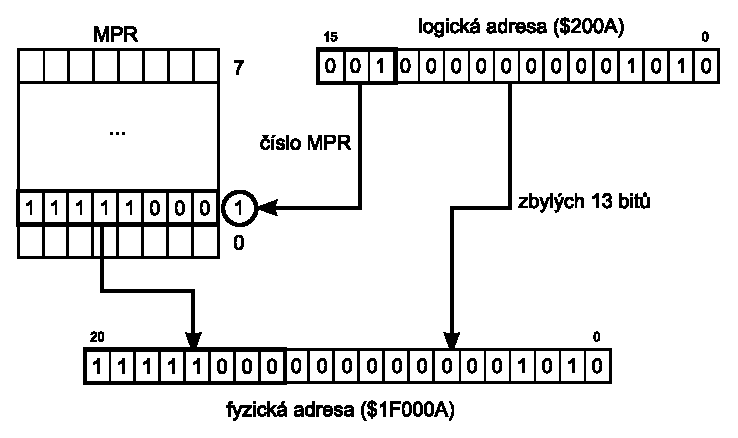
\includegraphics[width=12cm,height=7cm]{fig/pce_banks}
\caption{Výpočet fyzické adresy\label{fig:cpu_addr}}
\end{center}
\end{figure}

\newpage

% Instrukcni sada

\subsubsection{Instrukční sada}\label{chap:spec_hw_cpu_instr}

CPU HuC6280 rozšiřuje instrukční sadu WDC 65c02 (která je podrobně popsána,
včetně možnosti adresace operandů a vlivu na příznakový registr pro každou
instrukci, např. v \cite{www65c02}) o několik specifických instrukcí a způsobů
adresace operandů.

Jedná se o následující výčet instrukcí. Počty cyklů, možnosti adresace operandů
a vliv na příznakový registr pro jednotlivé instrukce lze nalézt v
\cite{Ormston06}.

\begin{description}
\item[{\sc bsr}] (Branch To Subroutine) \\
	Uloží absolutní adresu následující instrukce sníženou o jedna na zásobník a
	skočí do subrutiny.

\item[{\sc cla}] (Clear Accumulator) \\
	Nastaví hodnotu střadače na \uv{0}.

\item[{\sc clx}] (Clear Index X) \\
	Nastaví hodnotu indexového registru {\sf X} na \uv{0}.

\item[{\sc cly}] (Clear Index Y) \\
	Nastaví hodnotu indexového registru {\sf Y} na \uv{0}.

\item[{\sc csh}] (Clock Select High) \\
	Slouží ke změně obsahu skrytého registru {\sf CS} na \uv{1}. Procesor se přepne
	na kmitočet 7.16~MHz.

\item[{\sc csl}] (Clock Select Low) \\
	Slouží ke změně obsahu skrytého registru {\sf CS} na \uv{0}. Procesor se přepne
	na kmitočet 3.58~MHz.

\item[{\sc sax}] (Swap Accumulator And Index X) \\
	Prohodí obsah střadače a indexového registru {\sf X}.

\item[{\sc say}] (Swap Accumulator And Index Y) \\
	Prohodí obsah střadače a indexového registru {\sf Y}.

\item[{\sc set}] (Set Decimal Memory Operation Flag) \\
	Přepne procesor do akumulátorového módu (decimálního) na jeden instrukční
	cyklus (nastaví příznak \uv{T} na \uv{1}).

\item[{\sc sxy}] (Swap Index X And Index Y) \\
	Prohodí obsah indexových registrů {\sf X} a {\sf Y}.

\item[{\sc st0}] (Store At VDC Address 1) \\
	Zapíše data pro VDC HuC6270 do hardwarového registru 0 (fyzická adr. {\tt \$1FE000}).

\item[{\sc st1}] (Store At VDC Address 2) \\
	Zapíše data pro VDC HuC6270 do hardwarového registru 1 (fyzická adr. {\tt \$1FE002}).

\item[{\sc st2}] (Store At VDC Address 3) \\
	Zapíše data pro VDC HuC6270 do hardwarového registru 2 (fyzická adr. {\tt \$1FE003}).

\item[{\sc tai}] (Transfer 'from' Alternate 'to' Increment) \\
	Přenese blok dat z adresy {\it from} na adresu {\it to} tak, že v každém cyklu
	zamění adresu {\it from} s obsahem paměti na této adrese a zvýší adresu
	{\it to} o \uv{1}.

\item[{\sc tam}] (Transfer Accumulator To MPR) \\
	Přenese obsah střadače do mapovacího registru.

\item[{\sc tdd}] (Transfer 'from' Decrement 'to' Decrement) \\
	Přenese blok dat z adresy {\it from} na adresu {\it to} tak, že v každém cyklu
	obě adresy sníží o \uv{1}.

\item[{\sc tia}] (Transfer 'from' Increment 'to' Alternate) \\
	Přenese blok dat z adresy {\it from} na adresu {\it to} tak, že v každém cyklu
	sníží adresu {\it from} o \uv{1} a zamění adresu {\it to} s obsahem paměti
	na této adrese.

\item[{\sc tii}] (Transfer 'from' Increment 'to' Increment) \\
	Přenese blok dat z adresy {\it from} na adresu {\it to} tak, že v každém cyklu
	obě adresy zvýší o \uv{1}.

\item[{\sc tin}] (Transfer 'from' Increment 'to' Does Nothing) \\
	Přenese blok dat z adresy {\it from} na adresu {\it to} tak, že v každém cyklu
	zvýší adresu {\it from} o \uv{1}.

\item[{\sc tma}] (Transfer MPR To Accumulator) \\
	Přenese obsah mapovacího registru do střadače.

\item[{\sc tst}] (Test Bits) \\
	Otestuje bity mezi dvěma operandy kde jeden je přímý a jeden z paměti.
	Nastaví příznakový registr tak, že indikuje stav horních dvou bitů hodnoty
	načtené z paměti pomocí příznaků \uv{N} a \uv{O} a shodu alespoň v jednom
	bitu pomocí příznaku \uv{Z}.
\end{description}

\newpage

% Rezimy adresace operandů

\subsubsection{Režimy adresace operandů}\label{chap:spec_hw_cpu_addr}

Režimy adresace operandů instrukcí CPU HuC6280 jsou uvedeny v
tabulce~\ref{tab:cpu_addrmodes}. Většina instrukcí je použitelná jen s
několika ze všech vyjmenovaných způsobů adresace operandů, které v jejím
případě dávají smysl (např. jedinná instrukce, která může použít nepřímou
adresaci nebo nepřímou adresaci s indexem je {\sc jmp}). Způsoby adresace
operandů specifické pro CPU HuC6280 jsou uvedeny ve spodní části
tabulky~\ref{tab:cpu_addrmodes} oddělené čarou a popsány v následujícím textu.
Podrobnosti o jednotlivých způsobech adresace operandů lze nalézt v
\cite{www65c02, Ormston06}.

\begin{table}[h!]
\begin{center}
\begin{tabular}{|l|l|}
\hline
\textbf{Adresa} & \textbf{Syntaxe} \\
\hline
Implicitní (Implicite) &
	- \\
Střadačová (Accumulator) & 
	{\tt INS A} \\
Přímá (Immediate) &
	{\tt INS \#\$10} \\
Stránka nula (Zero page) &
	{\tt INS \$10} \\
Stránka nula s indexem (Zero page, X/Y) &
	{\tt INS \$10,X} nebo {\tt INS \$10,Y} \\
Relativní (Relative) &
	{\tt INS *+1} \\
Absolutní (Absolute) &
	{\tt INS \$1000}  \\
Absolutní s indexem (Absolute, X/Y) &
	{\tt INS \$1000,X} nebo {\tt INS \$1000,Y} \\
Nepřímá (Indirect) &
	{\tt INS (\$1000)} \\
Nepřímá stránkou nula (Indirect zero page) &
	{\tt INS (\$10)} \\
Nepřímá s indexem (Indirect, X/Y) &
	{\tt INS (\$10, X)} nebo {\tt INS (\$10),Y} \\
Absolutní nepřímá s indexem (Absolute Indirect, X) &
	{\tt INS (TBL, X)} \\
\hline
Přenosová (Transfer) &
	{\tt INS \$1000, \$2000, \#\$3000} \\
Přímá a stránka nula (Immediate and Zero page) &
	{\tt INS \#\$10, \$20} \\
Přímá a stránka nula s indexem X & \\
	\hspace{0.5cm}(Immediate and Zero page, X) &
	{\tt INS \#\$10, \$20, X} \\
Přímá a absolutní (Immediate and Absolute) &
	{\tt INS \#\$10, \$1000} \\
Přímá a absolutní s indexem X & \\
	\hspace{0.5cm}(Immediate and Absolute, X) &
	{\tt INS \#\$10, \$1000, X} \\
\hline
\end{tabular}
\end{center}
Pozn.: Instrukce {\sc ins} je smyšlená stejně jako všechny použité adresy a
návěstí. Přehled má sloužit pouze pro demonstraci zápisu v assembleru pro
CPU HuC6280.
\caption{Možnosti adresace operandů CPU HuC6280\label{tab:cpu_addrmodes}}
\end{table}


Režimy specifické pro CPU HuC6280 jsou obvykle spjaty s některou konkrétní
instrukcí nebo jejich skupinou. Tyto instrukce vyžadují adresaci operandů právě
jedním konkrétním způsobem. Jedná se o režimy popsané v následujícím výčtu
(včetně uvedení instrukcí, se kterými mohou být použity):

\begin{description}
\item[Přenosová adresa] (Transfer) \\
	Používá se pouze ve spojení s instrukcemi blokových přenosů ({\sc tai},
	{\sc tdd}, {\sc tia}, {\sc tii} a {\sc tin}), které očekávají tři operandy
	- absolutní adresu zdroje {\it from}, absolutní adresu cíle {\it to} a
	délku bloku.\\
%	\textbf{Příklad:}  {\tt TAI \$1234, \$5678, \#\$9ABC}

\item[Přímá adresa a stránka nula] (Immediate and Zero page) \\
	Tento způsob adresace se využívá jen s instrukcí {\sc tst}. Operandem je
	přímá hodnota a offset ve stránce nula. 
%	\textbf{Příklad:}  {\tt TST \$\#12, \$34}

\item[Přímá adresa a stránka nula s indexem X] (Immediate and Zero page, X) \\
	Tento způsob adresace se opět využívá jen s instrukcí {\sc tst}. Operandem
	je přímá hodnota a offset ve stránce nula s indexem X (adresa ve stránce
	nula zvýšenou o hodnotu indexového registru {\sf X}). 
%	\textbf{Příklad:}  {\tt TST \$\#12, \$34, X}

\item[Přímá adresa a absolutní adresa] (Immediate and Absolute) \\
	Tento způsob adresace se opět využívá jen s instrukcí {\sc tst}. Operandem
	je přímá hodnota a absolutní adresa. 
%	\textbf{Příklad:}  {\tt TST \$\#12, \$3456}

\item[Přímá adresa a absolutní adresa s indexem X] (Immediate and Absolute, X) \\
	Tento způsob adresace se opět využívá jen s instrukcí {\sc tst}. Operandem
	je přímá hodnota a absolutní adresa s indexem X (absolutní adresa zvýšená o
	hodnotu indexového registru {\sf X}). 
%	\textbf{Příklad:}  {\tt TST \$\#12, \$3456, X}
\end{description}

% Preruseni

\subsubsection{Přerušení}\label{chap:spec_hw_cpu_irq}

Přerušení procesoru je stav kdy procesor vyskočí ze sekvenčního zpracování
programu na předem určené místo (toto místo určuje speciální odskoková adresa,
tzv. \uv{vektor přerušení}) a zahájí zpracování přerušení obslužnou rutinou.
Seznam dostupných přerušení a jejich vektorů je uveden v
tabulce~\ref{tab:cpu_irq}.

\begin{table}[ht]
\begin{center}
\begin{tabular}{|c|l|}
\hline
\textbf{Přerušení} & \textbf{Vektor} \\
\hline
RESET & {\tt \$FFFE}\\
NMI & {\tt \$FFFC}\\
TIMER & {\tt \$FFFA}\\
IRQ1 & {\tt \$FFF8}\\
IRQ2 & {\tt \$FFF6}\\
\hline
\end{tabular}
\end{center}
\caption{Přerušení CPU HuC6280 a jejich vektory\label{tab:cpu_irq}}
\end{table}

\begin{description}
\item[RESET] - Přerušení vyvolané při každém spuštění procesoru.

\item[NMI] - Nemaskovatelné přerušení. Toto přerušení nastává i v případě že je
	pomocí příznakového registru P zakázáno zpracování přerušení (příznak
	\uv{I}). Procesor HuC6280 přerušení umí obsloužit a má pro něj vyhrazen
	vektor, ale dle \cite{MacDonald02} neexistuje způsob (pin přerušení není
	fyzicky s ničím propojen), jak by bylo možné ho vyvolat.

\item[TIMER] - Přerušení vyvolané interním časovačem procesoru HuC6280. K
	přerušení dochází v okamžiku kdy čítač časovače přeteče na maximální
	hodnotu čítáním z hodnoty 0.

\item[IRQ1] - Přerušení vyvolané pomocným grafickým procesorem VDC (HuC6270).

\item[IRQ2] - Přerušení vyvolané instrukcí {\sc brk}. \cite{MacDonald02} uvádí,
	že pin přerušení IRQ2 je vyveden do portu pro čipové karty HuCard a
	přerušení je sdíleno s některými hardwarovými rozšířeními konzole NEC
	PCEngine. Zda-li bylo přerušení vyvoláno softwarově instrukcí {\sc brk},
	nebo hardwarově lze zjistit pomocí příznaku \uv{B} příznakového registru
	{\sf P}.
\end{description}

Adresy určené ke čtení vstupně-výstupní vyrovnávací paměti při obsluze
přerušení jsou {\tt \$1400} a {\tt \$1401}. Přerušení mohou být, s vyjímkou
NMI, zakázána (maskována) pomocí příznaku \uv{I} příznakového registru {\sf P}
nebo pomocí zápisu na spodní tři bity na adrese {\tt \$1402}.

Všechna přerušení musí být po zpracování potvrzena libovolným zápisem na adresu
{\tt \$1403}. Pokud se tak nestane, bude přerušení (v případě že není zakázano)
nastávat po provedení každé instrukce.

% Periferni zarizeni

\subsubsection{Periferní zařízení}\label{chap:spec_hw_cpu_peripheral}

Všechna zařízení připojená k řídící sběrnici procesoru HuC6280 (jak interní
periférie typu paralelní I/O port či časovač, tak externí podpůrné grafické
procesory VDC HuC6270 a VCE HuC6260) s procesorem komunikují pomocí
vstupně-výstupní banky (tzv. \uv{I/O page}) {\tt \$FF}, do které mapují regiony
své paměti (registry atd.). Mapa této banky je uvedena v
tabulce~\ref{tab:cpu_iopage}

\begin{table}[h]
\begin{center}
\begin{tabular}{|c|l|}
\hline
\textbf{Logická adresa} & \textbf{Význam} \\
\hline
{\tt \$0000} - {\tt \$03FF} & VDC HuC6270 (viz.~\ref{chap:spec_hw_vdc}) \\
{\tt \$0400} - {\tt \$07FF} & VCE HuC6260 (viz.~\ref{chap:spec_hw_vce}) \\
{\tt \$0800} - {\tt \$0BFF} & PSG (viz.~\ref{chap:spec_hw_psg}) \\
{\tt \$0C00} - {\tt \$0FFF} & časovač \\
{\tt \$1000} - {\tt \$13FF} & paralelní I/O port \\
{\tt \$1400} - {\tt \$17FF} & jednotka obsluhy přerušení
	(viz.~\ref{chap:spec_hw_cpu_irq}) \\
{\tt \$1800} - {\tt \$1BFF} & {\em nevyužito} \\
{\tt \$1C00} - {\tt \$1FFF} & {\em nevyužito} \\
\hline
\end{tabular}
\end{center}
\caption{Mapa vstupně-výstupní banky \$FF CPU HuC6280\label{tab:cpu_iopage}}
\end{table}

\begin{description}
\item[Časovač] - Jedná se o interní časovač implementovaný pomocí 7-mi bitového
	zachytávacího (latch) registru. Časovač je řízen stejným zdrojem hodinového
	signálu jako celý procesor v \uv{rychlém} režimu (7.16~MHz) a NENÍ ovlivněn
	použitím instrukcí {\sc csl} a {\sc csh} pro změnu kmitočtu procesoru.
	Čítač časovače dekrementuje svojí hodnotu každých 1024 cyklů.

	Časovač je ovládán pomocí dvojice logických adres kde {\tt \$0C00} slouží k
	nastavení výchozí hodnoty zachytávacího registru časovače (nižších 6 bitů
	0-127) a {\tt \$0C01} slouží k aktivaci časovače (nejnižší bit). Přerušení
	TIMER je vyvoláno při přetečení hodnoty zachytávacího registru z
	hodnoty 0 do hodnoty 127.

\item[Paralelní I/O port] - standardní 8-mi bitový vstupně-výstupní port pro
	herní ovladač. Informace o stavu herního ovladače jsou dostupná pomocí
	logické adresy {\tt \$1000} kde čtením nižších 4 bitů získáme data o stavu
	herního ovladače podle tabulky~\ref{tab:cpu_ioport}. 

	V případě zápisu jsou zajímavé nejnižší dva bity. Na nejnižší se zapisuje
	stav \uv{SEL}. Hodnota \uv{0} vybírá čtení stavu čtveřice akčních tlačítek,
	hodnota \uv{1} pak čtení stavu čtveřice směrovek. Na druhý nejnižší bit se
	zapisuje stav \uv{CLR}, který v případě nastavení na 1 způsobí ignoraci
	ovladače.

	\begin{table}[ht]
	\begin{center}
	\begin{tabular}{|c|c|l|}
	\hline
	\textbf{Bit} & \textbf{Stav SEL} & \textbf{Tlačítko} \\
	\hline
	3 & 0 & tlačítko \uv{Start} \\
	2 & 0 & tlačítko \uv{Select} \\
	1 & 0 & tlačítko \uv{I.} \\
	0 & 0 & tlačítko \uv{II.} \\
	3 & 1 & směrový kříž, doleva \\
	2 & 1 & směrový kříž, dolů \\
	1 & 1 & směrový kříž, doprava \\
	0 & 1 & směrový kříž, nahoru \\
	\hline
	\end{tabular}
	\end{center}
	\caption{Kódování stavu herního ovladače na paralelním I/O portu CPU
		HuC6280\label{tab:cpu_ioport}}
	\end{table}
\end{description}

%
% VDC
%

\subsection{VDC}\label{chap:spec_hw_vdc}

Video Display Controller (VDC), neboli kontrolér pro zobrazení nese označení
HuC6270. Je to plně 16-ti bitový procesor s 20-ti 16-ti bitovými registry a
schopností adresovat až 128~KB video paměti. K VDC HuC6270 se přistupuje
prostřednictvím tří speciálních instrukcí {\sc st0}, {\sc st1} a {\sc st2}, a
vstupně-výstupní banky {\tt \$FF}. VDC HuC6270 zajišťuje generování výsledného
obrazu z dlaždic pozadí a sprajtů\footnote{Grafických symbolů poskládaných
zpravidla do popředí větší scény. Více o \uv{sprites} viz.
\cite{wwwWikiSprite}.}. Pro získání informace o barvách a jejich uspořádání do
barevných palet využívá druhého z dvojice grafických pomocných procesorů, Video
Color Encoder (VCE) - enkodér barev HuC6260 (viz.~\ref{chap:spec_hw_vce}).

Vzhledem k povaze herního systému NEC PCEngine byl zobrazovací systém navržen
pro připojení k televiznímu setu pomocí RF (anténního) výstupu. Veškerý
zobrazovací mechanismus je tedy přizpůsoben zobrazování na televizoru a
vykreslování na obrazovku tedy probíhá po řádcích\footnote{V případě současných
digitálních televizorů s LCD/TFT displejem samozřejmě probíhá vykreslování
jinak, než pomocí katodového paprsku na CRT televizorech. Nicméně i tyto
televizory jsou kompatibilní se standardy PAL a NTSC a tudíž po připojení
systému k RF (anténního) vstupu televizoru bude vše fungovat jak má z důvodu
zpětné kompatibility s analogovým signálem (pokud touto funkčností televizor
disponuje). Následující dva odstavce jsou zde uvedeny záměrně pro osvětlení
pojmu vertikální synchronizace.} (scanlines).

Řádky na stínítku televizní obrazovky jsou tvořeny dopadáním elektronů
vyslaných katodou obrazovky na mřížku a předáváním energie luminoforu, který se
v místě dopadu rozzáří a vytvoří světelný bod. Paprsek elektronů vysílaný
katodou obrazovky pochopitelně vykresluje jednotlivé řádky s prodlevou pro
navrácení na začátek dalšího řádku (tato prodleva se nazývá {\em horizontal
blanking}). Stejně tak nastává prodlení při návratu paprsku z pravého dolního
rohu obrazovky do levého horního - tedy po vykreslení celého jednoho snímku
(tato prodleva se nazývá {\em vertical blanking}).~\cite{Vit02}

Dění na obrazovce je s děním uvnitř logiky programu synchronizováno právě
pomocí tohoto údaje. Televizor samozřejmě nijak systému nepředává informaci o
každém vykreslení jednoho celého snímku, ale vzhledem k tomu, že je zobrazení
na televizoru standardizováno do norem PAL a NTSC, kde je pevně dán počet
snímku zobrazených za sekundu a počet řádků tvořících jeden snímek, je možné
přesně vypočítat čas synchronizace. Tato synchronizace je zpravidla prováděna
vyvoláním přerušení (a nazývá se {\em vertikální synchronizace}, neboli {\em
vertical synchronization}).

NEC PCEngine pracuje v režimu NTSC, který je definován 60-ti zobrazenými
proloženými (vykreslují se jen liché, nebo jen sudé řádky) snímky za sekundu
při 263 řádcích na jeden snímek.~\cite{Vit02}

% Parametry zobrazeni

\subsubsection{Parametry zobrazení}\label{chap:spec_hw_vdc_display}

VDC HuC6270 dokáže pracovat ve variabilním rozlišení obrazu. To se může měnit
za běhu programu modifikací registrů VDC HuC6270. Maximální horizontální
rozlišení je 512 pixelů (lze snížit po násobcích 8 pixelů), maximální
vertikální rozlišení je 240 pixelů (opět lze snížit po násobcích 8 pixelů).
Většina herních programů využívá rozlišení 256x224 pixelů. Ačkoliv je barevná
hloubka zobrazení 9 bitů (512 barev rozděleno na dvě skupiny separátních palet
pro dlaždice pozadí a sprajty), dokáže systém NEC PCEngine zobrazit najednou
maximálně 482 barev.~\cite{wwwWikiTurboGrafx, Schleussinger98}

Jak již bylo naznačeno, VDC HuC6270 generuje výsledný obraz ze dvou skupin
grafických elementů. Každá tato skupina představuje jednu z následujících
rovin:

\begin{description}
\item[dlaždic pozadí] velkých 8x8 pixelů. Každá z těchto dlaždic může používat
	až 16 barev z jedné z 16-ti palet určených pro dlaždice pozadí. Jedna z
	barev je stejná napříč všemi paletami.

\item[sprajtů] ve velikostech od 16x16 pixelů až 32x64 pixelů. Sprajtů může být
	zároveň zobrazeno maximálně 64 a každý z nich může používat až 15 barev z
	jedné z 16-ti palet určených pro sprajty. Jedna barva ve všech paletách je
	vždy transparentní.
\end{description}

Vykreslování roviny sprajtů i roviny dlaždic pozadí může být potlačeno
prostřednictvím zápisu do jednoho z registrů VDC HuC6270
(viz.~\ref{chap:spec_hw_vdc_regs}).

% Organizace videopameti

\subsubsection{Organizace videopaměti}\label{chap:spec_hw_vdc_vram}

Protože je videopaměť (VRAM) systému NEC PCEngine velká jen 64~KB, nemůže být
výsledný obraz uložen v podobě bitové mapy jako je tomu např. u PC. Nebylo by
totiž možné dosáhnout tak vysokých rozlišení při celkovém počtu barev.

Při nejvyšším rozlišení 512x240 pixelů a využití 8-mi bitové barevné hloubky by
uložení výsledné bitové mapy do paměti znamenalo: $512 * 240 * 8b = 983 040b ~=
120~KB$, což je zhruba dvojnásobek paměti kterou máme k dispozici. Namísto toho
jsou obrazová data rozdělena do dlaždic pozadí a sprajtů, ze kterých je obraz
výsledné scény poskládán (u dlaždic pozadí je pevně dána velikost 8x8 pixelů, u
sprajtů je velikost odkrokována po 16-ti pixelech v rozsahu 16x16 pixelů až
32x64 pixelů).

Dlaždice pozadí a sprajty jsou definovány pomocí dvou atributových tabulek:
Background Attribute Table ({\it BAT}) a Sprite Attribute Table ({\it SAT}),
které vycházejí z rozdělení výsledného obrazu na rovinu dlaždic pozadí a rovinu
sprajtů (viz. výše).

Podstatným činitelem z hlediska snížení nároků na pamět je způsob práce s
barvami. Konkrétně rozdělením barev do dvou skupin po 16-ti 16-ti barevných
paletách, kde index každé barvy lze zákodovat do 4 bitů (přijatelnou nevýhodou
je možnost použít jen 16 barev v rámci jedné dlaždice pozadí nebo sprajtu).
Obrazová data jsou v paměti uložena {\em planárním} způsobem (viz. dále).

\begin{description}
\item[BAT] - tabulka atributů dlaždic pozadí\\
	Tabulka {\it BAT} je uložena na začátku videopaměti (adresa {\tt \$00}) a
	její velikost je závislá na rozlišení (tj. na počtu zobrazených dlaždic
	pozadí). Pokud je tabulka kratší, než je velikost obrazovky, dojde při
	zpracování k přetečení na začátek a opakování tabulky (čehož lze s výhodou
	využít). Délka tabulky {\it BAT} je nastavována pomocí jednoho z registrů
	VDC HuC6270 (viz.~\ref{chap:spec_hw_vdc_regs}). Nejmenší možná velikost
	tabulky {\it BAT} je 32x32 dlaždic, největší pak 128x64 dlaždic. Tabulky
	generující rovinu dlaždic pozadí větší, než je fyzické rozlišení televizní
	obrazovky jsou využívány pro skrolování pozadí (které výsledné scéně dodává
	hloubku).

	Každým prvkem tabulky {\it BAT} je ukazatel do videopaměti o délce jednoho
	slova, které se skládá z indexu použité palety (vybírá jednu z 16-ti palet
	určených pro dlaždice pozadí) a indexu vzoru dlaždice pozadí. Adresu vzoru
	dlaždice pozadí ve videopaměti získáme vynásobením indexu vzoru dlaždice
	pozadí číslem 32 (bitový posun o 5 vlevo).

	Ukazatel má tvar popsaný v tabulce~\ref{tab:vdc_batword}. Vzhledem k
	velikosti videopaměti by index vzoru dlaždice pozadí neměl překročit číslo
	2048 (VDC HuC6270 má v případě NEC PCEngine jen polovinu videopaměti,
	kterou je schopen adresovat).~\cite{Schleussinger98}

	Uspořádání ukazatelů v tabulce {\it BAT} je zleva doprava, shora dolů (tak,
	jak budou dlaždice vykresleny do roviny dlaždic pozadí).

	\begin{table}[ht]
	\begin{center}
	\begin{tabular}{|l|l|}
	\hline
	\textbf{Bit} & \textbf{Význam} \\
	\hline
	15-12 & index palety \\
	11-0 & index vzoru \\
	\hline
	\end{tabular}
	\end{center}
	\caption{Tvar ukazatele na dlaždici pozadí v tabulce BAT VDC HuC6270
		HuC6270\label{tab:vdc_batword}}
	\end{table}

\item[SAT] - tabulka atributů sprajtů\\
	Tabulka {\it SAT} nemá, narozdíl od tabulky {\it BAT}, pevnou pozici ve
	videopaměti. Ukazatel na její začátek je uložen v jednom z registrů VDC
	HuC6270 (viz.~\ref{chap:spec_hw_vdc_regs}). Maximalní počet sprajtů
	(ukazatelů v tabulce {\it SAT}) je 64.

	Princip je stejný jako u tabulky {\it BAT}. Narozdíl od \uv{jednoduchých}
	dlaždic pozadí mají ale sprajty řadu atributů a lze na ně aplikovat několik
	transformací (např. zrcadlové otočení v obou osách). Proto je každému prvku
	tabulky {\it SAT}, tedy ukazateli na sprajt, vyhrazen prostor
	4 slova, kde nejnižší dvě slova udávají souřadnice sprajtu v rámci výsledné
	scény, následující slovo (odspoda) udává index vzoru sprajtu ve videopaměti
	a nejvyšší slovo je bitové pole atributů sprajtu. Adresu vzoru sprajtu ve
	videopaměti získáme vynásobením indexu vzoru sprajtu číslem 64 (bitový
	posun o 6 vlevo).
	
	Ukazatel má tvar popsaný v tabulce~\ref{tab:vdc_sat4word}. Vzhledem k
	velikosti videopaměti by index vzoru sprajtu neměl překročit číslo 512 (VDC
	má v případě NEC PCEngine jen polovinu paměti, kterou je schopen
	adresovat).~\cite{Schleussinger98}

	Pozice jednotlivých sprajtů ve scéně je uvedena přímo v tabulce {\it SAT}
	hodnotou slov 0 a 1. Vzhledem k povaze sprajtů nemá, narozdíl od dlaždic
	pozadí, uspořádání tabulky {\it SAT} vliv na pozici při vykreslování.

	\begin{table}[ht]
	\begin{center}
	\begin{tabular}{|c|l|l|}
	\hline
	\textbf{Slovo} & \textbf{Bit} & \textbf{Význam} \\
	\hline
	0
		& 15-10 & {\em nevyužito} \\
		& 9-0 & pozice v ose Y \\
	\hline
	1
		& 15-10 & {\em nevyužito} \\
		& 9-0 & pozice v ose X \\
	\hline
	2
		& 15-11 & {\em nevyužito} \\
		& 10-0 & index vzoru \\
	\hline
	3
		& 15 & zrcadlení v ose Y \\
		& 14 & {\em nevyužito} \\
		& 13-12 & výška sprajtu (CGY) \\
		& 11 & zrcadlení v ose X \\
		& 10-9 & {\em nevyužito} \\
		& 8 & šířka sprajtu (CGX)\\
		& 7 & priorita (SPBG) \\
		& 6-4 & {\em nevyužito} \\
		& 3-0 & index palety \\
	\hline
	\end{tabular}
	\end{center}
	\caption{Tvar ukazatele na sprajt v tabulce SAT VDC
		HuC6270\label{tab:vdc_sat4word}}
	\end{table}

	Význam jednotlivých atributů sprajtu uložených v bitovém poli v nejvyšším
	slově každého prvku tabulky {\it SAT} je následující:

	\begin{description}
	\item[zrcadlení v ose Y] - pixely sprajtu budou vykresleny zrcadlově v ose Y.

	\item[výška sprajtu (CGY)] - dvoubitový kód udávající výšku sprajtu danou
		hodnotou tohoto atributu (decimálně): \uv{0} pro 16 pixelů,
		\uv{1} pro 32 pixelů a \uv{3} pro 64 pixelů).

	\item[zrcadlení v ose X] - pixely sprajtu budou vykresleny zrcadlově v ose X.

	\item[šířka sprajtu (CGX)] - jednobitový kód udávající šířku sprajtu. Pro
		hodnotu \uv{0} bude mít sprajt šířku 16 pixelů, pro hodnotu \uv{1} pak 32 pixelů.

	\item[priorita (SPBG)] - pokud je priorita nastavena na hodnotu 0, pak jsou
		pixely sprajtu vykresleny jen v místech překryvu s průhlednými pixely
		dlaždic pozadí v rovině dlaždic pozadí.

	\item[index palety] - index palety, vybírá jednu ze 16-ti palet určených
		pro sprajty.
	\end{description}
\end{description}

Kromě atributových tabulek videopamět samozřejmě obsahuje i samotná obrazová
data dostupná pomocí indexu vzoru (dlaždice pozadí nebo sprajtu). Pomocí tohoto
indexu lze snadno spočítat adresu vzoru ve videopaměti. Samotný vzor je pak
uložen {\em planárním} způsobem na této adrese.

Planární způsob uložení obrazových dat je způsob, při kterém se data výsledného
obrazu ukládají po bitových rovinách (bitplanes) jejichž spojením vznikne index
barvy v paletě. Namísto toho, aby byl ve videopaměti obraz uložen v podobě
sledu indexů barev jednotlivých bodů, je v paměti uložen sled bitových rovin
představujících vždy informaci pro celý obraz (viz.
obr.~\ref{fig:vdc_planar}). Spojením informací ze všech rovin v jednom místě
obrazu pak dostaneme index barvy v paletě pro toto místo. Z předchozího popisu
plyne, že do $n$ bitových rovin zakódujeme $2^n$ barev.

\begin{figure}[ht]
\begin{center}
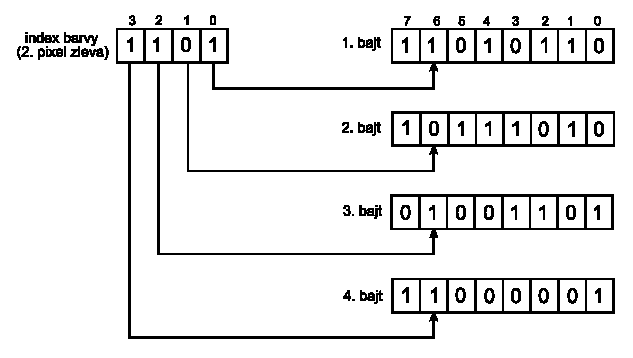
\includegraphics[width=10cm,height=5.4cm]{fig/pce_planar}
\caption{Planární způsob ukládání obrazových dat.\label{fig:vdc_planar}}
\end{center}
\end{figure}

V případě VDC HuC6270 systému NEC PCEngine index barvy uvádíme v rámci palety
určené ukazatelem v tabulce {\it BAT} nebo {\it SAT}. Každá z 16-ti palet (ať
už palet pro dlaždice pozadí, nebo palet pro sprajty) může obsahovat maximálně
16 barev, jejichž indexy zakódujeme pomocí 4 bitů. Pro uložení obrazových dat
zpracovávanhých VDC HuC6270 budou tedy potřeba 4 bitové roviny.

Vzory dlaždic pozadí jsou ve videopaměti reprezentovány jako 8 čtveřic bajtů
pro jednotlivé bitové roviny. Tyto čtveřice reprezentují jednotlivé řádky
vzoru. Každý vzor dlaždice pozadí ve videopaměti zabírá $8 * 8 * 4b = 256b / 8
= 32B$. VDC HuC6270 neočekává čtveřice bajtů ve videopaměti přímo za sebou, ale
proložené mezerou 16 bajtů (viz. obr.~\ref{fig:vdc_pat}). Více podrobností
lze nalézt např. v \cite{MacDonald02}.

\begin{figure}[ht]
\begin{center}

\includegraphics[width=11.5cm,height=4cm]{fig/pce_pixel}
\caption{Reprezentace vzoru dlaždice pozadí a vzoru sprajtu ve
videopaměti.\label{fig:vdc_pat}}
\end{center}
\end{figure}

Vzory sprajtů jsou ve videopaměti reprezentovány stejným způsobem jako vzory
dlaždic pozadí. Je však třeba vzít v úvahu několik drobných odlišností
týkajících se velikosti. Minimální velikost sprajtu je 16x16 pixelů, čtveřic
tedy není 8, ale 16 a pro jednotlivé řádky vzoru nejsou použity bajty ale
slova. Velikost jednoho vzoru sprajtu ve videopaměti je tedy $16 * 16 * 4b =
1024b / 8 = 128B$. VDC HuC6270 opět počítá s 16-ti bajtovým proložením ve
videopaměti (viz. obr.~\ref{fig:vdc_pat}).

Sprajty mohou navíc nabývat velikosti až 32x64 pixelů, což se řeší tak, že se
použijí sousední vzory sprajtů (ve skutečnosti se jedná přímo o maskování
pomocí atributů CGY a CGX). VDC HuC6270 se sprajtem větším než 16x16 pixelů
zachází z hlediska {\it SAT} úplně stejně, jako se sprajtem velkým 16x16 pixelů
(např. při použití atributu zrcadlového otočení v libovolné ose budou tedy
otočeny i příslušné okolní části sprajtu). Více podrobností lze nalézt např.
v~\cite{MacDonald02}.

% DMA

\subsubsection{Přímý přístup do paměti}\label{chap:spec_hw_vdc_dma}

VDC HuC6270 podporuje dva druhy přímého přístupu do paměti (Direct Memory
Access, DMA). Jedná se o:

\begin{itemize}
\item kopírování z videopaměti do videopaměti (dále jen VRAM/VRAM)
\item přesun z videopaměti do {\it SAT} (dále jen VRAM/{\it SAT})
\end{itemize}

Řízení DMA u VDC HuC6270 je prováděno pomocí čtveřice registrů {\sf DCR}, {\sf
SOUR}, {\sf DESR} a {\sf LENR}. Přenos je zahájen zápisem do registru {\sf
LENR}, který určuje délku bloku přenášeného z adresy uložené v registru {\sf
SOUR} na adresu uloženou v registru {\sf DESR}. Délka bloku může nabývat hodnot
0 pro 1B dlouhý blok, až po 65535 pro 64~KB dlouhý blok. Hodnoty jednotlivých
registrů slouží jako čítače a po dokončení se nenulují. Po ukončení libovolného
typu DMA přenosu může VDC HuC6270 vygenerovat přerušení IRQ1 (čtením ze
stavového registru VDC HuC6270 na logické adrese {\tt \$0000} jsme schopni
určit o jaký druh DMA se jednalo). Během DMA přenosu je stavový příznak VDC
HuC6270 \uv{čekání na CPU pro DMA (BSY)} nastaven na hodnotu \uv{1}.

% Registry

\subsubsection{Registry}\label{chap:spec_hw_vdc_regs}

VDC HuC6270 disponuje dvaceti registry o délce jednoho slova. K těmto registrům se
z CPU HuC6280 přistupuje pomocí tří speciálních instrukcí {\sc st0}, {\sc st1}
a {\sc st2} a vstupně-výstupní banky {\tt \$FF}
(viz.~\ref{chap:spec_hw_cpu_peripheral}). V té jsou namapovány tři důležité adresy
určené k čtení a zápisu do registrů VDC HuC6270. Jejich výčet a význam je uveden v
tabulce~\ref{tab:vdc_ffpage}. Detaily o významu jednotlivých bitů stavového
registru přístupného čtením log. adresy {\tt \$0000} lze nalézt např. v
\cite{MacDonald02}.

Zápis a čtení registrů VDC HuC6270 se provádí tak, že je zápisem spodních čtyř
bitů na logické adrese {\tt \$0000} nebo pomocí instrukce {\sc st0} zvolen
konkétní registr VDC HuC6270. Ten lze potom číst a zapisovat pomocí logických
adres {\tt \$0002} a {\tt \$0003}, nebo pomocí instrukcí {\sc st1} a {\sc st2}.
Dvojice adres pro zápis a čtení je použita, protože CPU HuC6280 je 8-mi bitový,
zatímco registry VDC HuC6270 jsou 16-ti bitové.

\begin{table}[ht]
\begin{center}
\begin{tabular}{|c|l|l|l|}
\hline
\textbf{Logická adresa} & \textbf{Operace} & \textbf{Bit} & \textbf{Význam} \\
\hline
	{\tt \$0000}
		& čtení
			& 7 & {\em nevyužito} \\
			& & 6 & čekání na CPU pro DMA (BSY) \\
			& & 5 & přerušení vertikální synchronizace (VD) \\
			& & 4 & přerušení \uv{konec DMA VRAM/VRAM} (DV) \\
			& & 3 & přerušení \uv{konec DMA VRAM/{\it SAT}} (DS) \\
			& & 2 & přerušení \uv{raster compare} (RR) \\
			& & 1 & přerušení přetečení sprajtů (OR) \\
			& & 0 & přerušení kolize sprajtu 0 (CR) \\
		& zápis
			& 7-5 & {\em nevyužito} \\
			& & 4-0 & offset registru VDC pro zápis/čtení \\
\hline
	{\tt \$0002}
		& čtení/zápis
		& 7-0 & méně významný bajt slova v registru VDC \\
\hline
	{\tt \$0003}
		& čtení/zápis
		& 7-0 & více významný bajt slova v registru VDC \\
\hline
\end{tabular}
\end{center}
	\caption{Adresy VDC HuC6270 ve vstupně-výstupní bance \$FF CPU
	HuC6280\label{tab:vdc_ffpage}}
\end{table}

Význam důležitých registrů je popsán v následujícím výčtu. Číslo uvedené za
slovem \uv{Registr} je offset registru, které se skutečně zapisuje na spodní
čtyři bity logické adresy {\tt \$0000}. Podrobné informace o jednotlivých
registrech lze nalézt např. v \cite{Schleussinger98}.

\begin{description}
\item[Registr {\tt \$00} {\sf MAWR}] (Memory Address Write) \\
	Čítač adresy při zápisu do videopaměti. Je nutné si uvědomit, že ačkoliv je
	VDC HuC6270 schopný adresovat 128~KB videopaměti, dostupných je v případě
	systému NEC PCEngine jen 64~KB, proto je poslední platnou adresou {\tt
	\$7FFF}.

\item[Registr {\tt \$01} {\sf MARR}] (Memory Address Read) \\
	Čítač adresy při čtení z videopaměti. Platí zde stejné adresní omezení jako
	v případě registru {\sf MAWR}.

\item[Registr {\tt \$02} {\sf VRR/VWR}] (VRAM Read/Write) \\
	Registr čtení/zápisu hodnoty z/do videopaměti na adrese udané hodnotou
	registru {\sf MARR}, příp. {\sf MAWR}. Při čtení více významného bajtu
	pomocí logické adresy {\tt \$0003} dochází k automatické inkrementaci
	registru {\sf MARR}. příp. {\sf MAWR}.

\item[Registr {\tt \$05} {\sf CR}] (Control Register) \\
	Konfigurační registr VDC HuC6270. Obsahuje bitové pole umožňující provádět
	řadu nastavení VDC HuC6270. Význam jednotlivých bitů (do kterého spadají
	příznaku) tohoto bitového pole je uveden v tabulce~\ref{tab:vdc_cr}. Význam
	jednotlivých příznaků uložených v tomto registru následuje:

	\begin{table}[ht]
	\begin{center}
	\begin{tabular}{|c|c|c|c|c|c|c|c|c|c|c|c|}
	\hline
	\textbf{Bit} & 15-13 & 12-11 & 10 & 9-8 & 7 & 6 & 5-4 & 3 & 2 & 1 & 0 \\
	\hline
	\textbf{Příznak} & ? & IW & ? & ? & BB & SB & ? & VB & RC & SO & SC \\
	\hline
	\end{tabular}
	\end{center}
		\caption{Význam bitů registru {\sf CR} VDC HuC6270\label{tab:vdc_cr}}
	\end{table}

	\begin{description}
	\item[IW] Hodnota těchto dvou bitů registru {\sf CR} určuje skok, o který
		se bude automaticky inkrementovat hodnota registru {\sf MAWR} po čtení
		významějšího slova (tj. čtení z logické adresy {\tt \$0003}). Hodnoty
		(decimálně):
		\begin{description}
		\item[{\tt 0}]: inkrementace o 1
		\item[{\tt 1}]: inkrementace o 32
		\item[{\tt 2}]: inkrementace o 64
		\item[{\tt 3}]: inkrementace o 128
		\end{description}

	\item[BB] Povolení/zákaz vykreslování roviny dlaždic pozadí.

	\item[SB] Povolení/zákaz vykreslování roviny sprajtů.

	\item[VB] Povolení/zákaz generování přerušení IRQ1 při \uv{vertical
		blanking}.

	\item[RC] Povolení/zákaz generování přerušení IRQ1 při \uv{raster
		compare}.

	\item[SO] Povolení/zákaz generování přerušení IRQ1 při překrytí sprajtů.

	\item[SC] Povolení/zákaz generování přerušení IRQ1 při kolizi sprajtu 0.
	\end{description}

\item[Registr {\tt \$06} {\sf RCR}] (Raster Compare) \\
	Obsah tohoto registru po součtu s číslem 64 určuje číslo řádku při kterém
	VDC HuC6270 vyvolá přerušení IRQ1 (pokud je toto povoleno 3 nejnižším bitem
	registru {\sf CR}).

\item[Registr {\tt \$07} {\sf BXR}] (Background Scroll X) \\
	Spodních deset bitů tohoto registru udává posun roviny dlaždic pozadí v ose
	X (je to offset v pixelech, nikoliv v počtu dlaždic jak mylně uvádí některé
	dokumenty).

\item[Registr {\tt \$08} {\sf BYR}] (Background Scroll Y) \\
	Spodních devět bitů tohoto registru udává posun roviny dlaždic pozadí v ose
	Y (opět jde o offset v pixelech).

\item[Registr {\tt \$09} {\sf MWR}] (Memory Width) \\
	Tento registr obsahuje bitové pole, které určuje velikost roviny dlaždic
	pozadí (ta může být větší než rozlišení obrazovky, čehož se často využívá
	při použití registrů {\sf BXR} a {\sf BYR}). Význam jednotlivých bitů v
	tomto bitovém poli je uveden v tabulce~\ref{tab:vdc_mwr}.

	\begin{table}[ht]
	\begin{center}
	\begin{tabular}{|l|l|l|l|}
	\hline
	\textbf{Bit} & \textbf{Význam} & \textbf{Hodnota} & \textbf{Šířka} \\
	\hline
	15-7 & {\em nevyužito} && \\
	6 & výška roviny dlaždic pozadí & 0 & 32 dlaždic \\
		& & 1 & 64 dlaždic \\
	5-4 & šířka roviny dlaždic pozadí & 00 & 32 dlaždic \\
		& & 01 & 64 dlaždic \\
		& & 10 & 128 dlaždic \\
		& & 11 & 128 dlaždic \\
	3-0 & {\em nevyužito} && \\
	\hline
	\end{tabular}
	\end{center}
		\caption{Význam bitů registru {\sf MWR} VDC HuC6270\label{tab:vdc_mwr}}
	\end{table}

\item[Registr {\tt \$0F} {\sf DCR}] (DMA Control) \\
	Tento registr slouží k řízení DMA přenosů. Význam jednotlivých bitů v tomto
	bitovém poli je uveden v tabulce~\ref{tab:vdc_dcr}. Bity 2 a 3 určují
	operaci na zdrojové/cílové adrese, která se bude vykonávat v každé iteraci
	blokového přenosu. Podrobnosti o DMA přenosech jsou uvedeny v
	sekci~\ref{chap:spec_hw_vdc_dma}.

	\begin{table}[ht]
	\begin{center}
	\begin{tabular}{|l|l|l|l|}
	\hline
	\textbf{Bit} & \textbf{Význam} & \textbf{Hodnota} & \textbf{Operace} \\
	\hline
	15-5 & {\em nevyužito} && \\
	4 & DSR DMA (opakování DMA přenosu z VRAM do {\em SAT}) && \\
	3 & Operace aplikovaná na cílovou adresu & 0 & snížení o 1 \\
		& & 1 & zvýšení o 1 \\
	2 & Operace aplikované na zdrojovou adresu & 0 & snížení o 1 \\
		& & 1 & zvýšení o 1 \\
	1 & Povolení/zákaz přerušení \uv{konec DMA VRAM/VRAM} && \\
	0 & Povolení/zákaz přerušení \uv{konec DMA VRAM/{\it SAT}} && \\
	\hline
	\end{tabular}
	\end{center}
		\caption{Význam bitů registru {\sf DCR} VDC HuC6270\label{tab:vdc_dcr}}
	\end{table}

\item[Registr {\tt \$10} {\sf SOUR}] (DMA Source Address) \\
	Tento registr slouží k nastavení zdrojové adresy DMA přenosu.

\item[Registr {\tt \$11} {\sf DESR}] (DMA Destination Address) \\
	Tento registr slouží k nastavení cílové adresy DMA přenosu.

\item[Registr {\tt \$12} {\sf LENR}] (DMA Block length Address) \\
	Tento registr slouží k nastavení délky přenášeného bloku při DMA přenosu.
	Zápis do tohoto registru automaticky zahajuje DMA přenos.

\item[Registr {\tt \$13} {\sf SATB}] (Sprite Attribute Table) \\
	Tento registr obsahuje ukazatel na počátek tabulky {\em SAT} ve
	videopaměti.
\end{description}

% Preruseni

\subsubsection{Přerušení}\label{chap:spec_hw_vdc_irq}

VDC HuC6270 může v závislosti na nastavení registrů {\sf CR} a {\sf DCR}
generovat přerušení IRQ1 v řadě případů. Tyto případy lze snadno odlišit pomocí
příznaků přerušení ve stavovém registru VDC HuC6270, který lze číst na logické
adrese {\tt \$0000}.

Významná přerušení, která může VDC HuC6270 generovat jsou uvedena v
následujícím výčtu. Pro přehlednost jsou přerušení uvedena pod názvem
příslušných příznaků stavového registru VDC HuC6270.

\begin{description}
\item[VD] (Vertical Blanking) \\
	Toto přerušení je generováno při {\em vertikální synchronizaci}. Používá se k
	jednoduchému synchronizování programového kódu a vykreslování obrazu.

\item[DV] (VRAM to VRAM DMA Transfer Completion) \\
	Toto přerušení je generováno při dokončení operace DMA kopírování z
	videopaměti do videopaměti (VRAM/VRAM).

\item[DS] (VRAM to SAT DMA Transfer Completion) \\
	Toto přerušení je generováno při dokončení operace DMA přesun z videopaměti
	do {\it SAT}.

\item[RR] (Raster Compare) \\
	Toto přerušení je generováno, když interní čítač řádek obrazovky nabyde
	hodnoty registru {\sf RCR} zvětšené o číslo 64. \cite{Schleussinger98}

\item[OR] (Sprite Overflow) \\
	Toto přerušení nastává pokud je v aktuálně vykreslované řádce více než 16
	sprajtů.

\item[CR] (Sprite 0 Collision) \\
	Toto přerušení nastává v případě, kdy se netransparentní pixel sprajtu s
	pořadovým číslem 0 (tj. prvního záznamu v tabulce {\it SAT}) překryje s
	netransparentním pixelem kteréhokoliv jiného sprajtu.
\end{description}

%
% VCE
%

\subsection{VCE}\label{chap:spec_hw_vce}

Video Color Encoder (VCE), neboli enkodér barev nese označení HuC6260 a
obstarává systému NEC PCEngine správu barev. Pomocí registrů VCE je možné měnit
barvy ve všech 32 paletách (16 palet pro dlaždice pozadí a 16 palet pro
sprajty).

% Palety

\subsubsection{Palety}\label{chap:spec_hw_vce_palette}

Jak již bylo uvedeno dříve, VDC HuC6270 a VCE HuC6260 pracují celkem s 512-ti
barvami uloženými v barevné tabulce. Prvních 256 záznamů je určeno výhradně pro
vykreslování dlaždic pozadí a zbývajících 256 záznamů, pak výhradně pro
vykreslování sprajtů. Logicky jsou barvy v tabulce uspořádány do dvou skupin
16-ti palet, kde každá paleta obsahuje 16 barev. Tyto palety jsou odkazovány
přímo v ukazatelích z atributových tabulek {\it BAT} a {\it SAT} spravovaných
VDC HuC6270.

Jednotlivé záznamy tabulky barev jsou slova obsahující barevnou informaci.
Tvar jednoho záznamu z barevné tabulky je uveden v tabulce~\ref{tab:vce_color}.
Indexace barev probíhá v rámci celé tabulky 9-ti bitovým indexem barvy (logické
rozdělení na palety a skupiny palet je vnímáno pouze při práci s tabulkami {\it 
BAT} a {\it SAT} v rámci VDC HuC620.

\begin{table}[ht]
\begin{center}
\begin{tabular}{|l|l|}
\hline
\textbf{Bit} & \textbf{Význam} \\
\hline
15-9 & {\em nevyužito} \\
8-6 & zelená \\
5-3 & červená \\
2-0 & modrá \\
\hline
\end{tabular}
\end{center}
\caption{Tvar záznamu v barevné tabulce VCE
	HuC6260\label{tab:vce_color}}
\end{table}

Palety obsahují několik speciálních barev, při jejichž použití musíme očekávat
jiné chování vykreslovacích mechanismů. Tyto speciální barvy jsou:

\begin{description}
\item[transparentní barva] - transparentní barvu mají pixely (dlaždice pozadí
	nebo sprajtu), které nemají být vykresleny. V případě dlaždice pozadí bude
	na jejich místě vykreslena {\em barva pozadí}, v případě sprajtu barva
	pixelu dlaždice pozadí ležícím v místě transparentního pixelu sprajtu
	(případně opět {\em barva pozadí}, pokud je i pixel dlaždice pozadí
	transparentní). Transparentní barva je umístěna na indexu 0 ve všech
	paletách dlaždic pozadí i sprajtů.

\item[barva pozadí] - barva, která je vykreslena na místě \uv{pod}
	transparentním pixelem dlaždice pozadí. Tato barva je umístěna v 0-té
	paletě pro dlaždice pozadí na indexu 0 (tato barva je vlastně transparentní
	barvou pro všechny palety dlaždic pozadí). Barvu na indexu 0 všech
	ostatních palet pro dlaždice pozadí není možné zobrazit.

\item[barva přesahu] - barva, která je vykreslována zpravidla mimo plochu
	aktivního obrazu. Jedinný případ, kdy je tato barva zobrazena na obrazovce
	je, když je pomocí registru {\sf CR} VDC HuC6270 zakázáno vykreslování obou
	rovin (dlaždic pozadí i sprajtů). Jedná se o barvu na indexu 0 v 0-té
	paletě pro sprajty. Barvu na indexu 0 barvu všech ostatních palet pro
	sprajty též není možné zobrazit.
\end{description}

% Registry

\subsubsection{Registry}\label{chap:spec_hw_vce_regs}

VCE mapuje své registry do adresního prostoru CPU HuC6280 pomocí čtveřice adres
v rámci stránky {\tt \$FF} (viz.~\ref{chap:spec_hw_cpu_peripheral}). Jejich výčet a
význam je uveden v tabulce~\ref{tab:vce_ffpage}. Práce s VCE HuC6260 je v
mnohém analogická s prací VDC HuC6270.

\begin{table}[ht]
\begin{center}
\begin{tabular}{|c|l|l|l|}
\hline
\textbf{Logická adresa} & \textbf{Význam} \\
\hline
	{\tt \$0402} & Index barvy v tabulce (méně významný bajt) \\
	{\tt \$0403} & Index barvy v tabulce (více významný bajt) \\
	{\tt \$0404} & Data (méně významný bajt) \\
	{\tt \$0405} & Data (více významný bajt) \\
\hline
\end{tabular}
\end{center}
	\caption{Adresy VCE HuC6260 ve vstupně-výstupní bance \$FF CPU
	HuC6280\label{tab:vce_ffpage}}
\end{table}

%
% PSG
%

\subsection{PSG}\label{chap:spec_hw_psg}

Programmable Sound Generator (PSG), tedy programovatelný generátor
zvuku, je jedno z periferních zařízení CPU HuC6280 osazené na stejném čipu.
Podrobně se jím zabývá např.~\cite{Clifford}.

PSG je vybaven šesti kanály, které jsou primárně určeny pro přehrávání 32
bajtových lineárních samplů s rozlišením 5 bitů. Některé kanály mohou být
využity k frekvenční modulaci\footnote{Možnost měnit aktuální nosnou frekvenci
přehrávaného signálu pomocí modulační amplitudy.} pomocí nízkofrekvenčního
oscilátoru (Low Frequency Oscillator, LFO), či generování bílého
šumu\footnote{Náhodný signál se stejným výkonem v pásmech se shodnou šířkou.
Využívá se k neumělé syntetizaci zvuku perkusí apod.} (White Noise). Každý z
kanálů může být také přepnut do módu přímého přístupu k datům (Direct Data
Access, DDA), kdy je zvuk programován přímo CPU HuC6280, což dovoluje např.
jednoduchou syntézu zvuku. Možnosti jednotlivých kanálů PSG jsou uvedeny v
tabulce~\ref{tab:psg_chan}.

V případě nastavení módu frekvenční modulace pro kanál 0 bude kanál 1 vždy
automaticky ztlumen.

\begin{table}[ht]
\begin{center}
\begin{tabular}{|c|l|}
\hline
\textbf{Kanál} & \textbf{Dostupné režimy} \\
\hline
	0 & samply, frekvenční modulace (podle kanálu 1), DDA \\
	1 & samply, frekvenční modulace (kanálu 0), DDA \\
	2 & samply, DDA \\
	3 & samply, DDA \\
	4 & samply, bílý šum, DDA \\
	5 & samply, bílý šum, DDA \\
\hline
\end{tabular}
\end{center}
	\caption{Možnosti jednotlivých kanálů PSG\label{tab:psg_chan}}
\end{table}

Ke zprocesování dat využívá PSG stejný zdroj hodin jako CPU HuC6280. Jedná se o
hodiny pevně nastavené na hodnotu 3.58~MHz nezávisle na stavu skrytého registru
{\sf CS} CPU HuC6280.

% Registry

\subsubsection{Registry}\label{chap:spec_hw_psg_regs}

Podobně jako VDC HuC6270, nebo VCE HuC6260 i PSG mapuje své registry do
adresního prostoru CPU HuC6280. Jedná se o deset adres v rámci stránky {\tt
\$FF} (viz.~\ref{chap:spec_hw_cpu_peripheral}). Jejich výčet a význam je uveden v
tabulce~\ref{tab:psg_ffpage}, kde jsou ve spodní části tabulky oddělené čarou
uvedeny registry ovlivněné hodnotou zapsanou na adresu {\tt \$8000}. Všechny
registry PSG jsou 8-mi bitové.

Nastavení hodnot registrů ovládajících režim (frekvenční modulace, generování
bílého šumu) u kanálu, kde tento režim není dostupný, bude PSG ignorováno.

\begin{table}[ht]
\begin{center}
\begin{tabular}{|c|l|l|l|}
\hline
\textbf{Logická adresa} & \textbf{Význam} \\
\hline
	{\tt \$0800} & Výběr kanálu (Channel Select) \\
	{\tt \$0801} & Globální vyvážení hlasitosti (Global Balance) \\
\hline
	{\tt \$0802} & Jemné nastavení frekvence (Fine Frequency Adjust) \\
	{\tt \$0803} & Hrubé nastavení frekvence (Rough Frequency Adjust) \\
	{\tt \$0804} & Režim kanálu (Channel Mode) \\
	{\tt \$0805} & Vyvážení hlasitosti (Channel Balance) \\
	{\tt \$0806} & Data \\
	{\tt \$0807} & Povolení a frekvence bílého šumu (Noise Control) \\
	{\tt \$0808} & Frekvence oscilátoru modulace (LFO Frequency) \\
	{\tt \$0809} & Povolení a ovládání oscilátoru modulace (LFO Control) \\
\hline
\end{tabular}
\end{center}
	\caption{Adresy PSG ve vstupně-výstupní bance \$FF CPU
	HuC6280\label{tab:psg_ffpage}}
\end{table}

\begin{description}
\item [Registr {\tt \$0800}] (Channel Select) \\
	Nastavením spodních 2 bitů se určuje, který z kanálů PSG bude použit
	při zápisech/čteních registrů {\tt \$0802} - {\tt \$0809}.

\item [Registr {\tt \$0801}] (Global Balance) \\
	Hodnota tohoto registru určuje globální hlasitost pro levý a pravý kanál v
	mezích hodnot 0-15. Pro nastavení globální hlasitosti pravého kanálu slouží
	spodní 4 bity, pro nastavení globální hlasitosti levého kanálu pak
	následující 4 bity. Tato hlasitost je aplikována až po smíšení všech kanálů
	v jejich konkrétních hlasitostech.

\item [Registry {\tt \$0802}] (Fine Frequency Adjust) a
	{\tt \$0803} (Rough Frequency Adjust) \\
	Frekvence je v případě PSG 12-ti bitové číslo. Spodní 4 bity registru {\tt
	\$0803} představují vrchní 4 bity a hodnota registru {\tt \$0802}
	zbývajících 8 bitů tohoto čísla. Pro převod na Hz lze použít následující
	vztah: $$ f = \frac{3580000}{32 * 12bit} Hz $$ což je dáno způsobem práce
	s frekvencí v režimu přehrávání samplů. V tomto režimu se jedná o ukazatel,
	který je dekrementován o 1 celkem 3580000-krát za sekundu a ukazuje přímo
	do dat samplu.

\item [Registr {\tt \$0804}] (Channel Control) \\
	Tento registr slouží jako bitové pole určené ke konfiguraci parametrů
	zvoleného kanálu. Význam jednotlivých bitů je popsán v
	tabulce~\ref{tab:psg_cr}.

	\begin{table}[ht]
	\begin{center}
	\begin{tabular}{|l|l|}
	\hline
	\textbf{Bit} & \textbf{Význam} \\
	\hline
		7 & Kanál zapnut/vypnut \\
		6 & DDA režim zapnut/vypnut \\
		5 & {\em nevyužito} \\
		4-0 & Celková hlasitost kanálu \\
	\hline
	\end{tabular}
	\end{center}
		\caption{Význam bitů registru {\tt \$0804} PSG\label{tab:psg_cr}}
	\end{table}

\item [Registr {\tt \$0805}] (Channel Balance) \\
	Tento registr slouží k nastavení vyvážení hlasitosti zvoleného kanálu.
	Pracuje analogicky s registrem {\tt \$0801}.

\item [Registr {\tt \$0806}] (Data) \\
	Spodních 5 bitů tohoto registru slouží k zápisu dat na zvolený kanál.
	Chování registru je rozdílné podle zvoleného režimu kanálu (viz. bity 7 a 6
	registru {\tt \$0804}).

	V běžném případě se do tohoto registru zapisují data samplu. V případě, že
	je na kanálu povoleno DDA, pak jsou data zapsaná do tohoto registu přímo
	mixována s ostatními kanály. V případě, že je zvolen kanál 1, je neaktivní
	a DDA je vypnuto, slouží tento registr k zápisu modulační vlny (více viz.
	\cite{Clifford}).

\item [Registr {\tt \$0807}] (Noise Control) \\
	Tento registr slouží k zapnutí a vypnutí generátoru bílého šumu a nastavení
	jeho frekvence. Použití tohoto registru má význam pouze v případě kanálů 4
	a 5. Registr je uspořádán jako bitové pole s bity významu popsaného v
	tabulce~\ref{tab:psg_noise}. Frekvence bílého šumu nastavovaná pomocí
	spodních 5-ti bitů je vyjádřena vzorcem (podrobnosti o původu vzorce lze
	nalézt v \cite{Clifford}): $$ f = \frac{3580000}{64 * 5bit} Hz $$

	\begin{table}[ht]
	\begin{center}
	\begin{tabular}{|l|l|}
	\hline
	\textbf{Bit} & \textbf{Význam} \\
	\hline
		7 & Bílý šum zapnut/vypnut \\
		6-5 & {\em nevyužito} \\
		4-0 & Frekvence šumu \\
	\hline
	\end{tabular}
	\end{center}
		\caption{Význam bitů registru {\tt \$0807} PSG\label{tab:psg_noise}}
	\end{table}

\item [Registr {\tt \$0808}] (LFO Frequency) \\
	V případě, že je kanál 0 v režimu frekvenční modulace, slouží tento registr
	u kanálu 1 k modelování frekvence modelovací vlny (definované registry {\tt
	\$0802} a {\tt \$0803} při vybraném kanálu 1. Frekvence daná tam uloženým
	12-ti bitovým číslem je vynásobena frekvencí LFO uloženou v tomto registru
	před dalším zpracováním.

\item [Registr {\tt \$0809}] (LFO Control) \\
	Tento registr slouží k ovládání parametrů frekvenční modulace kanálu 0
	kanálem 1. Jedná se o bitové pole, kde význam jednotlivých bitů je uveden v
	tabulce~\ref{tab:psg_lfo}. Více informací o programování oscilátoru
	frekvenční modulace je uvedeno v \cite{Clifford}.

	\begin{table}[ht]
	\begin{center}
	\begin{tabular}{|l|l|}
	\hline
	\textbf{Bit} & \textbf{Význam} \\
	\hline
		7 & Oscilátor modulace zapnut/vypnut \\
		6-2 & {\em nevyužito} \\
		1-0 & Režim oscilátoru modulace \\
	\hline
	\end{tabular}
	\end{center}
		\caption{Význam bitů registru {\tt \$0809} PSG\label{tab:psg_lfo}}
	\end{table}

\end{description}

%
% ROM
%

\subsection{Obraz ROM}\label{chap:spec_hw_rom}

Obraz ROM je binární otisk obsahu paměti v paměťovém modulu na čipové kartě
HuCard do souboru. Lze jej pořídit pomocí speciálního zařízení (např. PCE Pro
32M na obr.~\ref{fig:pce_pcepro32}), které sekvenčně adresuje a čte jednotlivé
bloky paměti připojené čipové karty HuCard a pomocí speciálního software
komunikujícího se zařízením pomocí standardního rozhraní (USB, paralelní port)
je ukládá do souboru na disku PC.

\begin{figure}[ht]
\begin{center}
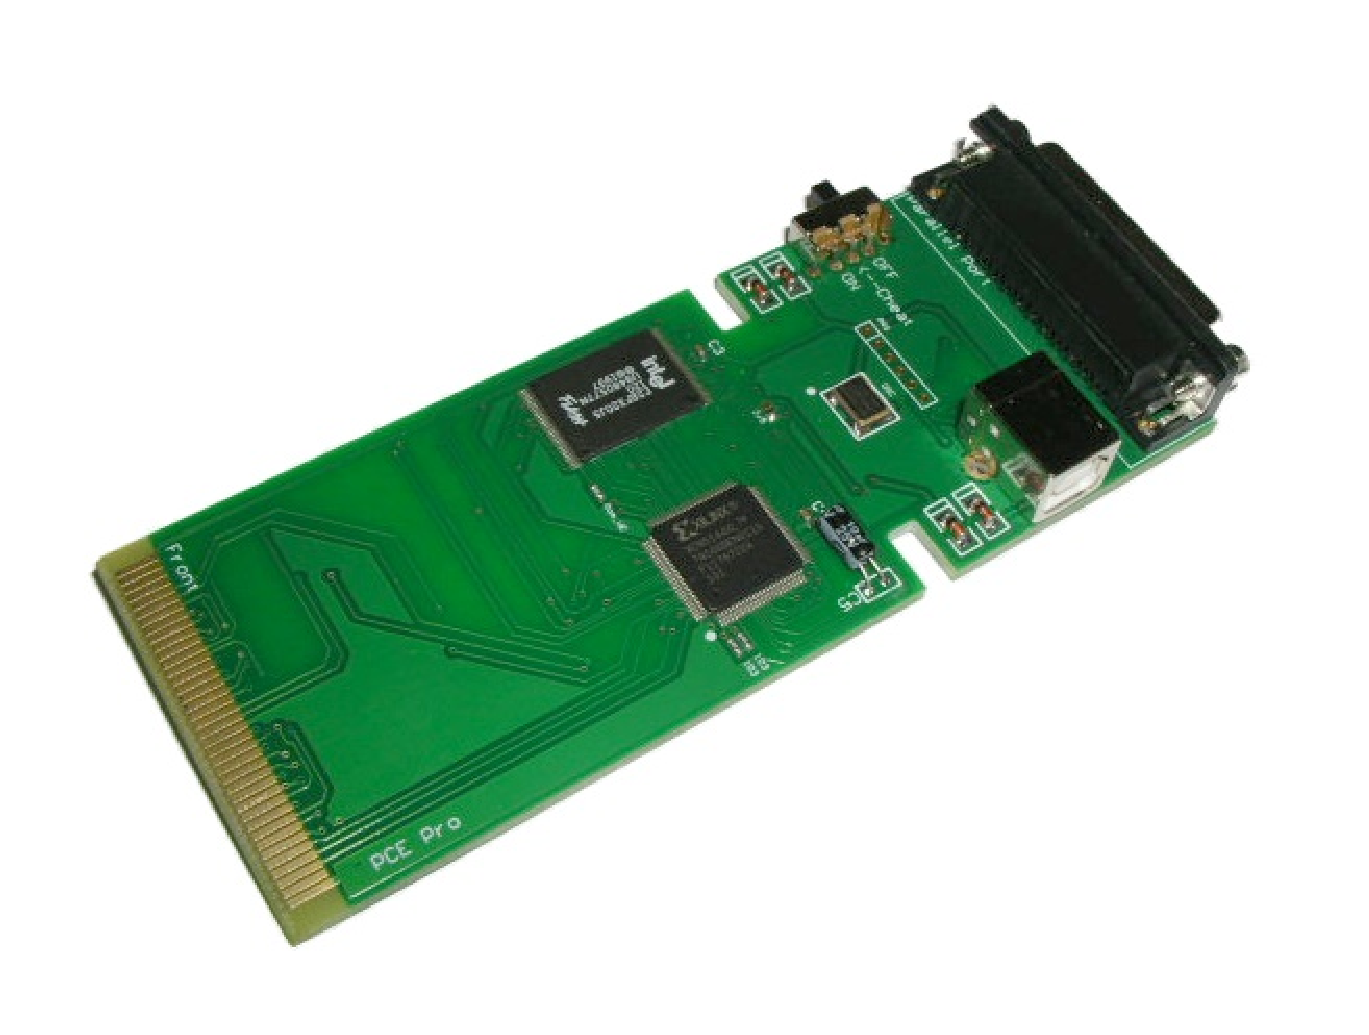
\includegraphics[width=6cm]{fig/pce_pcepro32}
\caption{PCE Pro 32M\label{fig:pce_pcepro32}}
\end{center}
\end{figure}

V nepříliš široké komunitě zabývající se emulací systému NEC PCEngine se
ustálil formát souboru s obrazem ROM použitý prvním emulátorem tohoto systému
(MagicEngine,~\cite{wwwMagicEngine}). Tento formát se vyznačuje absencí
jakýchkoliv metadat, kromě volitelné 512 bajtové hlavičky v úvodu souboru,
kterou lze snadno detekovat lichým počtem 512 bajtových bloků v souboru s
obrazem ROM.

Speciálním případem obrazu ROM jsou poměrně často používané obrazy o velikosti
384~KB. Tyto obrazy musí být rozděleny na dvě části umístěné v paměti ROM podle
schématu naznačeného v tabulce~\ref{tab:rom_split}.

\begin{table}[h!]
\begin{center}
\begin{tabular}{|l|l|l|}
\hline
\textbf{Offset v souboru} & \textbf{Délka} & \textbf{Offset v ROM} \\
\hline
	{\tt \$00000} & {\tt \$40000} & {\tt \$00000} \\
	{\tt \$40000} & {\tt \$20000} & {\tt \$80000} \\
\hline
\end{tabular}
\end{center}
	\caption{Schéma rozdělení 384~KB obrazů ROM\label{tab:rom_split}}
\end{table}

Maximální velikost paměťového modulu v čipové kartě HuCard je v základní
specifikaci omezena na 1~MB, minimální velikost není určena.

% -----------------------------------------------------------------------------
% Software NEC PCEngine
% -----------------------------------------------------------------------------

\section{Software}\label{chap:spec_sw}

Za dobu působení společnosti NEC v oblasti videoherního průmyslu, od roku 1987
do roku 1998, vznikla pro systém NEC PCEngine řada titulů. Jak samotný účel
systému předurčuje, majoritní většina byly herní programy. Kromě původních
titulů se společnost NEC snažila získat uživatele videoherních systémů na svou
stranu vydáním některých titulů, které se proslavily na systému Nintendo NES,
jako např. {\em Castlevania} nebo {\em StreetFighter}. Řada titulů vydaných
právě pro NEC PCEngine je přehledně katalogizována na~\cite{wwwPceCP}.
